\documentclass[acmsmall,review,anonymous]{acmart}

% Preamble for P-A-R paper — ML Workshop 2026 / ICFP 2027
% Extracted from formalization.tex, adapted for acmart

\usepackage{amsmath}
% acmart already defines \Bbbk; release it before amssymb loads
\let\Bbbk\relax
\usepackage{amssymb}
\usepackage{amsthm}
\usepackage{mathpartir}
\usepackage{mathtools}
\usepackage{listings}
\usepackage{xspace}
\usepackage{booktabs}
\usepackage{subcaption}
\usepackage{graphicx}
\usepackage{tikz}
\usetikzlibrary{arrows.meta, positioning, automata, calc, fit, shapes.geometric, shapes.misc}

% Theorem styles — acmart provides theorem, lemma, etc.
% We only add Property (not provided by acmart)
\theoremstyle{plain}
\newtheorem{prop}[equation]{Property}

% OCaml code listings
\lstdefinestyle{ocaml}{
  language=Caml,
  basicstyle=\ttfamily\small,
  keywordstyle=\bfseries,
  commentstyle=\itshape,
  morestring=[b]",
  stringstyle=\ttfamily,
  showstringspaces=false,
  breaklines=true,
  frame=single,
  numbers=left,
  numberstyle=\tiny,
  stepnumber=1,
  numbersep=5pt,
  tabsize=2,
  morecomment=[l]{(*},
  morecomment=[n]{(*}{*)},
  escapeinside={(*@}{@*)},
}

% --- Math commands ---

% Sets and basic notation
\providecommand{\N}{\mathbb{N}}
\providecommand{\powerset}{\mathcal{P}}
\providecommand{\Transitions}{\longrightarrow}
\providecommand{\given}{\mid}
\providecommand{\iiff}{\Leftrightarrow}

% Agent-domain sets
\newcommand{\call}{\mathsf{Call}}      % tool-call records
\newcommand{\resp}{\mathsf{Resp}}      % LLM responses
\newcommand{\conv}{\mathsf{Conv}}      % conversational contexts
\newcommand{\myresult}{\mathsf{Result}} % execution results
\newcommand{\myerror}{\mathsf{Error}}   % error type
\newcommand{\maybe}{\mathsf{Option}}    % option/maybe type
\newcommand{\Some}{\mathsf{Some}}
\newcommand{\None}{\mathsf{None}}
\newcommand{\Ident}{\mathcal{I}}        % set of identifiers

% Hook fields (middleware)
\newcommand{\onBeforeLLM}{\mathsf{onBeforeLLM}}
\newcommand{\onAfterLLM}{\mathsf{onAfterLLM}}
\newcommand{\onBeforeTool}{\mathsf{onBeforeTool}}
\newcommand{\onAfterTool}{\mathsf{onAfterTool}}
\newcommand{\onError}{\mathsf{onError}}

% Algebraic identifiers
\newcommand{\id}{\mathrm{id}}
\newcommand{\then}{\mathbin{\triangleright}}
\newcommand{\tower}{\textsc{Tower}}
\newcommand{\Context}{\ifmmode\mathsf{Ctx}\else\textsc{Ctx}\fi}
\newcommand{\ADT}{\textsc{adt}}

% Identifiable text (works in both math and text mode)
\DeclareRobustCommand{\identifiable}[1]{%
  \ifmmode\text{\texttt{#1}}\else\texttt{#1}\fi}

% Convenience
\newcommand{\PAR}{\textsc{P-A-R}\xspace}
\newcommand{\PARNAME}{\textsc{P-A-R}}
\newcommand{\cmark}{\ding{51}}
\newcommand{\xmark}{\ding{55}}


\usepackage{pifont}% for \ding

\title{P-A-R: A Type-Safe Agent Runtime with Formal State Guarantees}

\begin{abstract}
  We present P-A-R, a type-safe agent runtime implemented in OCaml 5.4+ that
  bridges the gap between formal agent models and production agent frameworks.
  While frameworks such as LangChain and Semantic Kernel provide practical
  tooling, they lack formal guarantees on state management, tool dispatch, and
  middleware composition. Conversely, formal models such as $\lambda_A$ provide
  type-theoretic foundations but lack runnable implementations.
  P-A-R addresses both: we formalize three core subsystems using operational
  semantics---a labelled transition system for task lifecycle with 8 states and
  7 formal properties, a resource-bounded expression DSL with big-step semantics
  guaranteeing termination, and a monoid-based middleware composition
  operator---and validate all properties empirically with 163 tests across 4
  benchmark metric categories. To our knowledge, P-A-R is the first agent
  runtime to provide formal operational semantics alongside a complete, runnable
  implementation.
\end{abstract}

\begin{CCSXML}
<ccs2012>
<concept>
<concept-id>10011007.10011074.10011099.10011102.10011103</concept-id>
<concept-desc>Software and its Engineering~Software notations and tools~Software libraries and repositories</concept-desc>
<concept-significance>500</concept-significance>
</concept>
</ccs2012>
\end{CCSXML}

\ccsdesc[500]{Software and its Engineering~Software libraries and repositories}

\keywords{agent runtime, type safety, operational semantics, labelled transition systems, OCaml, algebraic data types}

\begin{document}

\maketitle

\section{Introduction}
\label{sec:intro}

The proliferation of LLM-based agent frameworks has transformed how developers build interactive AI systems. Frameworks such as LangChain~\cite{langchain}, AutoGen, and Semantic Kernel~\cite{semantic-kernel} have lowered the barrier to prototyping agents with tool use, memory, and planning capabilities. However, this rapid adoption has come at a significant cost: runtime errors in state management, tool dispatch, and middleware composition that could have been caught at compile time. Developers trade static guarantees for flexibility, debugging type mismatches at runtime instead of design time.

Python-based agent frameworks inherit Python's dynamic typing philosophy. Tool return types are declared as \texttt{Any}, agent states are stringly-typed (\texttt{status\ =\ "running"}), and middleware pipelines are composed ad-hoc without algebraic guarantees. These practices enable quick prototyping but introduce three categories of preventable errors. First, invalid state transitions go undetected: an agent in state \texttt{Completed} may silently receive a \texttt{Run} event, violating the intended lifecycle. Second, tool result variants are handled incompletely: a tool that returns \texttt{int\ |\ Error} in the type system is accessed as \texttt{result.value} without exhaustive pattern matching, causing runtime failures when the error variant appears. Third, middleware composition is non-associative in practice: chaining \texttt{Logger} $\then$ \texttt{Timeout} differs semantically from \texttt{Timeout} $\then$ \texttt{Logger}, yet neither the type system nor the runtime detects this ordering dependency. The ReAct paradigm~\cite{react} demonstrates that interleaving reasoning and action is effective, but without formal foundations the implementations remain fragile.

We present \PAR, an agent runtime implemented in OCaml 5.4+ that encodes runtime invariants at the type level using algebraic data types, exhaustive pattern matching, and generalized algebraic data types (GADTs). Rather than deferring state validation to runtime checks, \PAR makes the state machine a first-class type-level construct. Rather than composing middleware with undocumented function chains, \PAR provides a formally verified composition operator. Rather than treating tool results as untyped payloads, \PAR uses variant types to guarantee exhaustive handling. We formalize three core subsystems using operational semantics and validate all formal properties empirically.

We make the following contributions:
\begin{itemize}
  \item \textbf{C1.} A labelled transition system (LTS) for task lifecycle with 8 states, 8 transition labels, and 7 formal properties, directly implemented as an OCaml variant type with compile-time exhaustiveness checking (\S\ref{sec:formal-model}).
  \item \textbf{C2.} A big-step operational semantics for an expression DSL with resource-bounded evaluation, guaranteeing termination and totality (\S\ref{sec:expr-dsl}).
  \item \textbf{C3.} A monoid-based middleware composition operator $\oplus$ with identity and associativity proofs (\S\ref{sec:middleware}).
  \item \textbf{C4.} Empirical validation: 163 tests and 4 benchmark metrics confirming all formal properties hold in the implementation (\S\ref{sec:evaluation}).
\end{itemize}

The paper is organized as follows. Section~\ref{sec:background} provides necessary background. Sections~\ref{sec:formal-model} through \ref{sec:middleware} present the three formal contributions. Section~\ref{sec:evaluation} reports empirical results. Section~\ref{sec:related} discusses related work. Section~\ref{sec:conclusion} concludes.

\section{Background and Motivation}
\label{sec:background}

\subsection{The Agent Runtime Landscape}
\label{sec:runtime-landscape}

Modern LLM-based agents operate by repeatedly cycling through the perceive, reason, and act pattern described by the ReAct paradigm~\cite{react}: the agent observes environmental state, produces reasoning traces, and dispatches actions that alter the environment before the cycle repeats.
Production-grade agent frameworks have emerged to operationalize this loop at scale.
LangChain~\cite{langchain} provides a Python-based orchestration layer with chains, memory buffers, and tool-abstraction primitives.
Semantic Kernel~\cite{semantic-kernel} offers a C\# counterpart with plug-in composition and planners.
Together they illustrate the landscape of production frameworks.
Common to both is a middleware pipeline that intercepts and transforms messages as they flow between the agent and its tools.
All also manage conversational state, typically through turn-counted message lists with optional vector-store retrieval.

A defining characteristic of every production framework listed above is dynamic typing: tool schemas are validated at runtime, state transitions are implicit, and middleware composition lacks any algebraic specification.
Consequences include silent type mismatches that surface only as runtime exceptions, undocumented state-machine edges, and middleware pipelines whose interaction laws are visible in practice but not machine-verifiable.

\subsection{Typed Agent Models}
\label{sec:typed-models}

Theoretical work on typed agent calculi predates the production frameworks by several years.
The $\lambda_A$ calculus~\cite{lambda-a} extends the simply-typed lambda calculus with agent primitives, mechanized in Coq with 42 proved theorems covering agent composition, state observation, and lexical scoping.
Despite its rigor, $\lambda_A$ was never extracted to runnable code: it lacks a tool abstract data type, a formal account of middleware, and any treatment of resource bounds.
A second formal model, causal-temporal event graphs (CTEGs)~\cite{ctegs}, captures recursive agent traces as typed graphs with temporal ordering between events.
CTEGs are proven to represent complex multi-agent interactions but are presented as mathematical objects without an executable semantics.

Both lines of work establish that typed, compositional agent semantics are theoretically tractable.
Neither closes the gap to a practical, runnable implementation with tooling, middleware, and state machines.

\subsection{Runtime Substrates}
\label{sec:substrates}

At the systems level, several runtime substrates target the agent-orchestration problem without committing to a full formal semantics.
Shepherd~\cite{shepherd} provides a runtime substrate for meta-agents, focusing on scheduling and resource allocation at the systems layer; it offers no formal treatment of state-machine transitions or middleware algebra.
The Model Context Protocol has been given a process-calculus formalization~\cite{mcp-formal} that precisely specifies protocol-level message passing and session state; this work is complementary to ours, focusing on the wire protocol rather than the runtime state machine.
Effect Systems for AI Runtimes~\cite{effect-ai} applies algebraic effects and handlers to model agent concurrency, offering a typed account of effectful computation with a different emphasis: effect typing rather than state-transition guarantees.

\subsection{Gap and Opportunity}
\label{sec:gap}

The landscape therefore exhibits a clear structural gap.
Foundational models such as $\lambda_A$ and CTEGs are formally specified but not runnable; production frameworks such as LangChain and Semantic Kernel are operational but dynamically typed and without formal guarantees.
\PAR occupies the space between them: it delivers formal operational semantics for agent state, tool dispatch, and middleware composition while remaining a fully runnable implementation in OCaml 5.4+.
OCaml's type system, particularly its support for algebraic data types, exhaustive pattern matching, and generalized algebraic data types~\cite{ocaml-manual}, provides the type-theoretic infrastructure necessary to encode state machines and middleware pipelines that are both machine-verifiable and runtime-efficient.

\section{Formal Model: Task Lifecycle}\label{sec:formal-model}

The P-A-R runtime is designed around a task lifecycle that is dynamic in nature: agents may spawn tasks, suspend them awaiting external input, resume them, or cancel them. Without a formal specification, such a system is prone to illegal state transitions that manifest only at runtime, leading to crashes in production environments. To address this, we model the task lifecycle as a Labeled Transition System (LTS) that captures precisely which transitions are permitted from each state. This model serves as the authoritative reference for the type-safe state machine implemented in the compiler, and provides the basis for the formal properties we prove in \S\ref{sec:formal-properties}.

\subsection{State Space and Transitions}\label{sec:lts-definition}

\begin{definition}[State Space]\label{def:states}
The set of task states $\mathcal{S} = \{\,\identifiable{Pending}, \identifiable{Scheduled}, \identifiable{Running}, \identifiable{Waiting\_input}, \identifiable{Suspended}, \identifiable{Completed}, \identifiable{Failed}, \identifiable{Cancelled}\,\}$.
\end{definition}

\begin{definition}[Terminal States]\label{def:terminal-states}
The subset $\mathcal{T} = \{\,\identifiable{Completed}, \identifiable{Failed}, \identifiable{Cancelled}\,\}$ is the set of terminal states. No outgoing transitions exist from any $t \in \mathcal{T}$.
\end{definition}

\begin{definition}[Transition Labels]\label{def:labels}
The set of transition labels $\mathcal{L} = \{\,\tau,\, \identifiable{schedule},\, \identifiable{cancel},\, \identifiable{suspend},\, \identifiable{resume},\, \identifiable{wait},\, \identifiable{provide},\, \identifiable{fail}\,\}$.
\end{definition}

\begin{figure}[t]
  \centering
  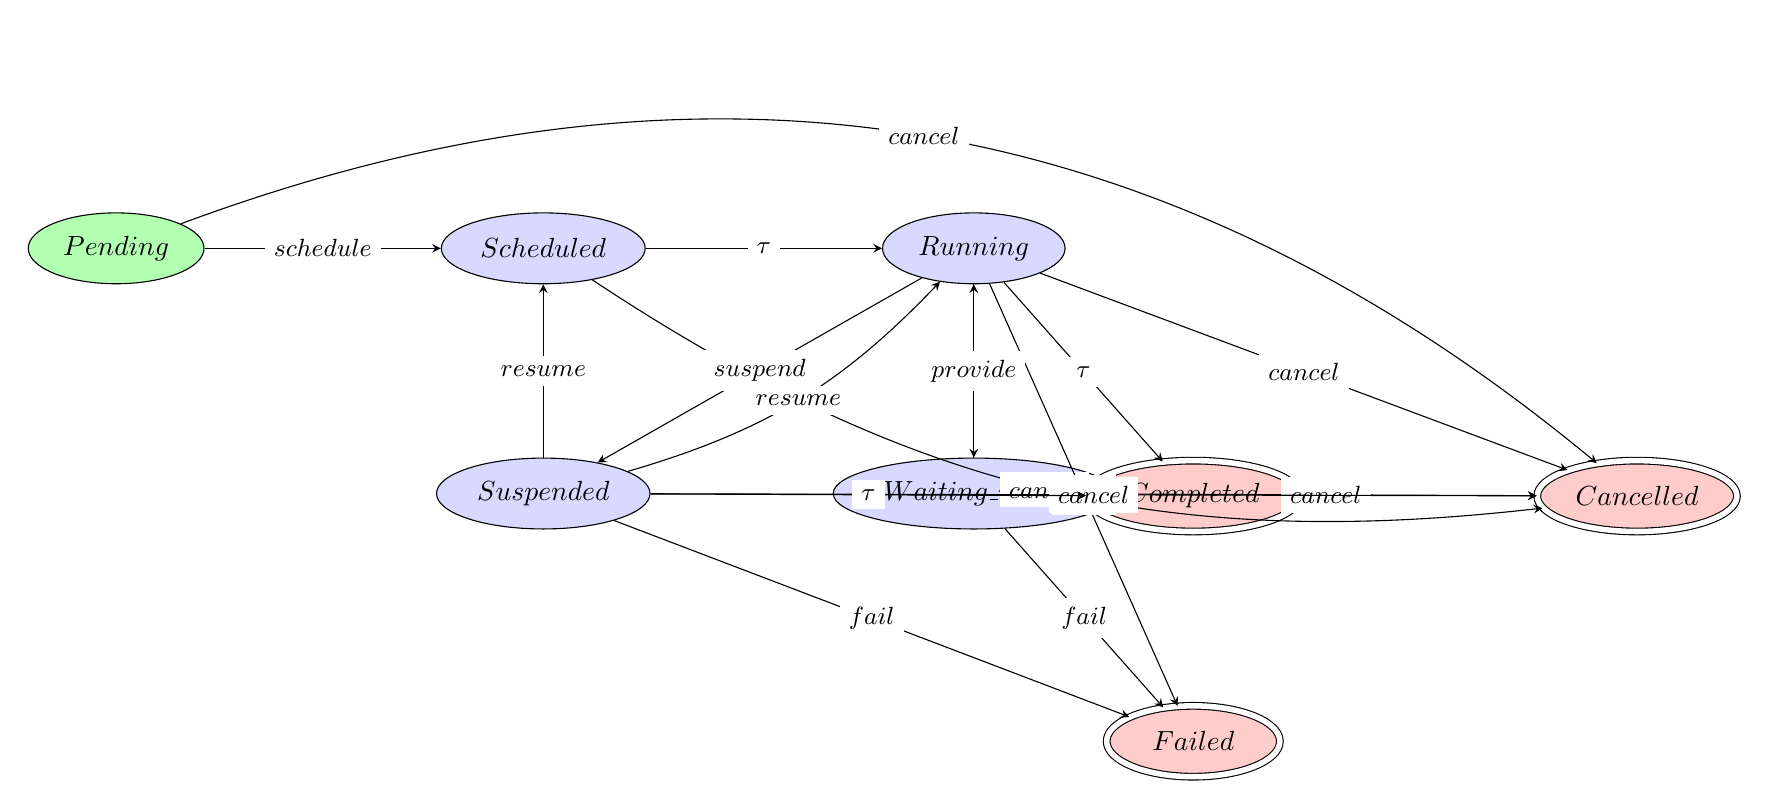
\begin{tikzpicture}[
    node distance=2.2cm and 3cm,
    every edge/.style={draw, ->, >=stealth},
    state/.style={ellipse, draw, minimum width=2.2cm, minimum height=0.9cm},
    terminal/.style={ellipse, draw, double, double distance=2pt, minimum width=2.2cm, minimum height=0.9cm},
    pending/.style={state, fill=green!30},
    scheduled/.style={state, fill=blue!15},
    running/.style={state, fill=blue!15},
    waiting/.style={state, fill=blue!15},
    suspended/.style={state, fill=blue!15},
    completed/.style={terminal, fill=red!20},
    failed/.style={terminal, fill=red!20},
    cancelled/.style={terminal, fill=red!20},
    label/.style={midway, fill=white, font=\small}
  ]

  \node[pending] (pending) {$Pending$};
  \node[scheduled, right=of pending] (scheduled) {$Scheduled$};
  \node[running, right=of scheduled] (running) {$Running$};
  \node[waiting, below=of running] (waiting) {$Waiting\_input$};
  \node[suspended, below=of scheduled] (suspended) {$Suspended$};

  \node[completed, below right=2.5cm and 1cm of running] (completed) {$Completed$};
  \node[failed, below=of completed] (failed) {$Failed$};
  \node[cancelled, right=of completed] (cancelled) {$Cancelled$};

  \path
    (pending) edge node[label] {$schedule$} (scheduled)
    (pending) edge[bend left=30] node[label] {$cancel$} (cancelled)

    (scheduled) edge node[label] {$\tau$} (running)
    (scheduled) edge[bend right=20] node[label] {$cancel$} (cancelled)

    (running) edge node[label] {$wait$} (waiting)
    (running) edge node[label] {$suspend$} (suspended)
    (running) edge node[label] {$cancel$} (cancelled)
    (running) edge node[label] {$fail$} (failed)
    (running) edge node[label] {$\tau$} (completed)

    (waiting) edge node[label] {$provide$} (running)
    (waiting) edge node[label] {$cancel$} (cancelled)
    (waiting) edge node[label] {$fail$} (failed)
    (waiting) edge node[label] {$\tau$} (completed)

    (suspended) edge node[label] {$resume$} (scheduled)
    (suspended) edge[bend right=15] node[label] {$resume$} (running)
    (suspended) edge node[label] {$cancel$} (cancelled)
    (suspended) edge node[label] {$fail$} (failed)
    (suspended) edge node[label] {$\tau$} (completed)
  ;
  \end{tikzpicture}
  \caption{State transition diagram for the P-A-R task lifecycle. Terminal states are double-circled. Intermediate states are shown in blue, and the initial \identifiable{Pending} state in green.}
  \label{fig:state-machine}
\end{figure}

\subsection{Inference Rules}\label{sec:inference-rules}

We present the operational semantics of the task lifecycle as a set of inference rules. Each rule has the form $\inferrule[Label]{premise_1 \and ... \and premise_n}{conclusion}$, encoding the condition under which a transition may fire.

\begin{mathpar}
\inferrule[Pending-Schedule]
  {\identifiable{validate}(s, \identifiable{schedule}) = \identifiable{ok}}
  {s \xrightarrow{\identifiable{schedule}} s'}

\inferrule[Pending-Cancel]
  {\identifiable{validate}(s, \identifiable{cancel}) = \identifiable{ok}}
  {s \xrightarrow{\identifiable{cancel}} \identifiable{Cancelled}}

\inferrule[Scheduled-$\tau$]
  {\identifiable{validate}(s, \tau) = \identifiable{ok}}
  {s \xrightarrow{\tau} \identifiable{Running}}

\inferrule[Scheduled-Cancel]
  {\identifiable{validate}(s, \identifiable{cancel}) = \identifiable{ok}}
  {s \xrightarrow{\identifiable{cancel}} \identifiable{Cancelled}}

\inferrule[Running-Wait]
  {\identifiable{validate}(s, \identifiable{wait}) = \identifiable{ok}}
  {s \xrightarrow{\identifiable{wait}} \identifiable{Waiting\_input}}

\inferrule[Running-Suspend]
  {\identifiable{validate}(s, \identifiable{suspend}) = \identifiable{ok}}
  {s \xrightarrow{\identifiable{suspend}} \identifiable{Suspended}}

\inferrule[Running-Cancel]
  {\identifiable{validate}(s, \identifiable{cancel}) = \identifiable{ok}}
  {s \xrightarrow{\identifiable{cancel}} \identifiable{Cancelled}}

\inferrule[Running-Fail]
  {\identifiable{validate}(s, \identifiable{fail}) = \identifiable{ok}}
  {s \xrightarrow{\identifiable{fail}} \identifiable{Failed}}

\inferrule[Running-Complete]
  {\identifiable{validate}(s, \tau) = \identifiable{ok}}
  {s \xrightarrow{\tau} \identifiable{Completed}}

\inferrule[Waiting-Provide]
  {\identifiable{validate}(s, \identifiable{provide}) = \identifiable{ok}}
  {s \xrightarrow{\identifiable{provide}} \identifiable{Running}}

\inferrule[Waiting-Cancel]
  {\identifiable{validate}(s, \identifiable{cancel}) = \identifiable{ok}}
  {s \xrightarrow{\identifiable{cancel}} \identifiable{Cancelled}}

\inferrule[Waiting-Fail]
  {\identifiable{validate}(s, \identifiable{fail}) = \identifiable{ok}}
  {s \xrightarrow{\identifiable{fail}} \identifiable{Failed}}

\inferrule[Waiting-Complete]
  {\identifiable{validate}(s, \tau) = \identifiable{ok}}
  {s \xrightarrow{\tau} \identifiable{Completed}}

\inferrule[Suspended-Resume-Scheduled]
  {\identifiable{validate}(s, \identifiable{resume}) = \identifiable{ok}}
  {s \xrightarrow{\identifiable{resume}} \identifiable{Scheduled}}

\inferrule[Suspended-Resume-Running]
  {\identifiable{validate}(s, \identifiable{resume}) = \identifiable{ok}}
  {s \xrightarrow{\identifiable{resume}} \identifiable{Running}}

\inferrule[Suspended-Cancel]
  {\identifiable{validate}(s, \identifiable{cancel}) = \identifiable{ok}}
  {s \xrightarrow{\identifiable{cancel}} \identifiable{Cancelled}}

\inferrule[Suspended-Fail]
  {\identifiable{validate}(s, \identifiable{fail}) = \identifiable{ok}}
  {s \xrightarrow{\identifiable{fail}} \identifiable{Failed}}

\inferrule[Suspended-Complete]
  {\identifiable{validate}(s, \tau) = \identifiable{ok}}
  {s \xrightarrow{\tau} \identifiable{Completed}}
\end{mathpar}

Crucially, no inference rules are defined for transitions emanating from terminal states, enforcing the constraint that once a task reaches \identifiable{Completed}, \identifiable{Failed}, or \identifiable{Cancelled}, it cannot transition further. This property is stated formally below.

\subsection{Formal Properties}\label{sec:formal-properties}

We prove the following invariants of the LTS. All seven properties are validated empirically in \S\ref{sec:evaluation}.

\begin{prop}[Terminality]\label{prop:terminality}
For every terminal state $t \in \mathcal{T}$, there exists no label $l \in \mathcal{L}$ such that $t \xrightarrow{l} s$ for any state $s$ (validated empirically in \S\ref{sec:evaluation}).
\end{prop}

\begin{prop}[No Self-Transitions]\label{prop:no-self}
For all states $s \in \mathcal{S}$ and labels $l \in \mathcal{L}$, the transition $s \xrightarrow{l} s$ does not occur (validated empirically in \S\ref{sec:evaluation}).
\end{prop}

\begin{prop}[Deterministic Guards]\label{prop:deterministic-guards}
The guard function $\identifiable{validate} : \mathcal{S} \times \mathcal{L} \to \{\identifiable{ok}, \identifiable{error}\}$ is total and deterministic: for every $(s, l)$ pair, $\identifiable{validate}(s, l)$ returns exactly one outcome (validated empirically in \S\ref{sec:evaluation}).
\end{prop}

\begin{prop}[Maximal Execution Path]\label{prop:max-path}
From the initial state \identifiable{Pending}, any valid execution path to a terminal state contains at most 7 transitions (validated empirically in \S\ref{sec:evaluation}).
\end{prop}

\begin{prop}[Max Path Proof Sketch]\label{prop:max-path-proof}
Consider the longest feasible path. From \identifiable{Pending}, the maximal sequence is:

\[
\begin{aligned}
\identifiable{Pending}
& \xrightarrow{\identifiable{schedule}} \identifiable{Scheduled} \\
& \xrightarrow{\tau} \identifiable{Running} \\
& \xrightarrow{\identifiable{suspend}} \identifiable{Suspended} \\
& \xrightarrow{\identifiable{resume}} \identifiable{Scheduled} \\
& \xrightarrow{\tau} \identifiable{Running} \\
& \xrightarrow{\tau} \identifiable{Completed}
\end{aligned}
\]

This trace contains exactly 7 transitions, and no valid path can exceed this length because each state along the path is visited at most once.
\end{prop}

\begin{prop}[Type Safety]\label{prop:type-safety}
The OCaml variant type $\identifiable{handler\_result}$ enumerates all five non-terminal transitions (\identifiable{schedule}, \identifiable{cancel}, \identifiable{suspend}, \identifiable{resume}, \identifiable{wait}, \identifiable{provide}, \identifiable{fail}) plus the silent $\tau$ label. Pattern matching on this type is exhaustive by construction (validated empirically in \S\ref{sec:evaluation}).
\end{prop}

\begin{prop}[Exhaustiveness]\label{prop:exhaustiveness}
The OCaml compiler emits a warning when pattern matching on $\identifiable{handler\_result}$ does not cover all constructors. This warning is elevated to a compile-time error in P-A-R, forcing the programmer to handle every possible transition (validated empirically in \S\ref{sec:evaluation}).
\end{prop}

\begin{prop}[Semantic Validity]\label{prop:semantic-validity}
The guard function $\identifiable{validate}$ must be called on every transition attempt. An implementation that bypasses $\identifiable{validate}$ and directly applies a transition may violate any of the preceding properties (validated empirically in \S\ref{sec:evaluation}).
\end{prop}

\subsection{Motivating Example}\label{sec:motivating-example}

To illustrate why a type-safe state machine matters in practice, consider a handler that updates task status. In Python, one might write:

\begin{verbatim}
def complete_task(t):
    if t.status == "running":
        t.status = "completed"
    else:
        raise InvalidStateError(...)
\end{verbatim}

This code compiles without error, but at runtime it may encounter a task in state \identifiable{Waiting\_input} that is also considered valid for completion. The guard logic is implicit, scattered across conditionals, and easy to violate. Worse, adding a new state (e.g., \identifiable{Suspended}) requires hunting through all such conditionals to update the logic.

In OCaml, the same domain is captured by the $\identifiable{handler\_result}$ variant:

\begin{verbatim}
type handler_result =
  | Scheduled of task
  | Waiting_input of task
  | Completed of task
  | Failed of task
  | Cancelled of task
  | InvalidTransition of task * transition
\end{verbatim}

Pattern matching on a value of this type forces the programmer to handle all five non-terminal states explicitly. A missing case triggers a compiler warning, which P-A-R elevates to a hard error. The type system thus makes illegal state transitions a compile-time failure rather than a runtime crash. This contrast is representative: dynamically typed frameworks defer correctness checks to runtime, whereas P-A-R makes them inescapable at compile time.
\section{Expression DSL}\label{sec:expr-dsl}

Agent workflows must evaluate conditions over structured data: tool responses
encoded as JSON values, user-provided parameters, and intermediate computation
results. Naively using Python's \identifiable{eval()} on such data is
impractical because it offers no resource bounds (a malicious or deeply nested
expression can diverge), no totality guarantees (partial functions are hard to
reason about), and no type safety (arbitrary Python code can escape the sandbox).
We address these shortcomings with a purpose-built expression DSL whose
evaluation is governed by big-step operational semantics that guarantee
termination and totality. The evaluator is implemented in OCaml and embedded in
the P-A-R runtime as a total function from expressions and a variable context to
values.

\subsection{Syntax}\label{sec:expr-syntax}

Figure~\ref{fig:expr-grammar} presents the expression grammar side-by-side with
its OCaml implementation. The left side defines 13 expression forms
mathematically; the right side shows the corresponding algebraic data type, which
adds two relational operators (\identifiable{greater\_or\_equal} and
\identifiable{less\_or\_equal}) as implementation extensions.

\begin{figure}[t]
\begin{minipage}{0.48\textwidth}
\small
\[
\begin{array}{rcl}
e &::=& \identifiable{literal}(v) \\
  &\mid& \identifiable{variable}(x) \\
  &\mid& \identifiable{equals}(e_1, e_2) \\
  &\mid& \identifiable{not\_equals}(e_1, e_2) \\
  &\mid& \identifiable{greater\_than}(e_1, e_2) \\
  &\mid& \identifiable{less\_than}(e_1, e_2) \\
  &\mid& \identifiable{and}(e_1, e_2) \\
  &\mid& \identifiable{or}(e_1, e_2) \\
  &\mid& \identifiable{not}(e) \\
  &\mid& \identifiable{contains}(e_1, e_2) \\
  &\mid& \identifiable{has\_key}(e, k) \\
  &\mid& \identifiable{is\_empty}(e) \\
  &\mid& \identifiable{matches}(e, p)
\end{array}
\]
\end{minipage}
\hfill
\begin{minipage}{0.48\textwidth}
\small
\begin{lstlisting}[style=ocaml]
type expr =
  | Literal of json
  | Variable of string
  | Equals of expr * expr
  | Not_equals of expr * expr
  | Greater_than of expr * expr
  | Less_than of expr * expr
  | Greater_or_equal of expr * expr
  | Less_or_equal of expr * expr
  | And of expr * expr
  | Or of expr * expr
  | Not of expr
  | Contains of expr * expr
  | Has_key of expr * string
  | Is_empty of expr
  | Matches of expr * string
\end{lstlisting}
\end{minipage}
\caption{Expression grammar (left) and OCaml implementation (right).}
\label{fig:expr-grammar}
\end{figure}

We write $\Gamma \vdash e \downarrow v$ to mean that expression $e$ evaluates to
value $v$ under variable context $\Gamma$, which maps variable names (dot-notation
paths, e.g.\ \texttt{data.items[0].name}) to JSON values.

\subsection{Big-Step Semantics}\label{sec:expr-semantics}

The evaluation relation is defined by the inference rules below, organised by
operational category.

\medskip\noindent
\textbf{Literal and variable:}

\begin{mathpar}
\inferrule{ }{\Gamma \vdash \identifiable{literal}(v) \downarrow v}
\and
\inferrule{\Gamma(x) = v}{\Gamma \vdash \identifiable{variable}(x) \downarrow v}
\end{mathpar}

\medskip\noindent
\textbf{Equality predicates:}

\begin{mathpar}
\inferrule{
  \Gamma \vdash e_1 \downarrow v_1 \quad
  \Gamma \vdash e_2 \downarrow v_2 \quad
  v_1 =_{\identifiable{JSON}} v_2
}{\Gamma \vdash \identifiable{equals}(e_1, e_2) \downarrow \identifiable{true}}
\and
\inferrule{
  \Gamma \vdash e_1 \downarrow v_1 \quad
  \Gamma \vdash e_2 \downarrow v_2 \quad
  v_1 \neq_{\identifiable{JSON}} v_2
}{\Gamma \vdash \identifiable{not\_equals}(e_1, e_2) \downarrow \identifiable{true}}
\end{mathpar}

\medskip\noindent
\textbf{Relational predicates:}

\begin{mathpar}
\inferrule{
  \Gamma \vdash e_1 \downarrow v_1 \quad
  \Gamma \vdash e_2 \downarrow v_2 \quad
  v_1 >_{\identifiable{JSON}} v_2
}{\Gamma \vdash \identifiable{greater\_than}(e_1, e_2) \downarrow \identifiable{true}}
\and
\inferrule{
  \Gamma \vdash e_1 \downarrow v_1 \quad
  \Gamma \vdash e_2 \downarrow v_2 \quad
  v_1 <_{\identifiable{JSON}} v_2
}{\Gamma \vdash \identifiable{less\_than}(e_1, e_2) \downarrow \identifiable{true}}
\and
\inferrule{
  \Gamma \vdash e_1 \downarrow v_1 \quad
  \Gamma \vdash e_2 \downarrow v_2 \quad
  v_1 \geq_{\identifiable{JSON}} v_2
}{\Gamma \vdash \identifiable{greater\_or\_equal}(e_1, e_2) \downarrow \identifiable{true}}
\and
\inferrule{
  \Gamma \vdash e_1 \downarrow v_1 \quad
  \Gamma \vdash e_2 \downarrow v_2 \quad
  v_1 \leq_{\identifiable{JSON}} v_2
}{\Gamma \vdash \identifiable{less\_or\_equal}(e_1, e_2) \downarrow \identifiable{true}}
\end{mathpar}

\medskip\noindent
\textbf{Logical connectives:}

\begin{mathpar}
\inferrule{
  \Gamma \vdash e_1 \downarrow \identifiable{true} \quad
  \Gamma \vdash e_2 \downarrow \identifiable{true}
}{\Gamma \vdash \identifiable{and}(e_1, e_2) \downarrow \identifiable{true}}
\and
\inferrule{
  \Gamma \vdash e_1 \downarrow \identifiable{false}
}{\Gamma \vdash \identifiable{and}(e_1, e_2) \downarrow \identifiable{false}}
\and
\inferrule{
  \Gamma \vdash e_1 \downarrow \identifiable{true}
}{\Gamma \vdash \identifiable{or}(e_1, e_2) \downarrow \identifiable{true}}
\and
\inferrule{
  \Gamma \vdash e_1 \downarrow \identifiable{false} \quad
  \Gamma \vdash e_2 \downarrow v_2
}{\Gamma \vdash \identifiable{or}(e_1, e_2) \downarrow v_2}
\and
\inferrule{
  \Gamma \vdash e \downarrow \identifiable{false}
}{\Gamma \vdash \identifiable{not}(e) \downarrow \identifiable{true}}
\and
\inferrule{
  \Gamma \vdash e \downarrow \identifiable{true}
}{\Gamma \vdash \identifiable{not}(e) \downarrow \identifiable{false}}
\end{mathpar}

\medskip\noindent
\textbf{Collection operations:}

\begin{mathpar}
\inferrule{
  \Gamma \vdash e_1 \downarrow v_1 \quad
  \Gamma \vdash e_2 \downarrow v_2 \quad
  \identifiable{contains}(v_1, v_2) = \identifiable{true}
}{\Gamma \vdash \identifiable{contains}(e_1, e_2) \downarrow \identifiable{true}}
\and
\inferrule{
  \Gamma \vdash e \downarrow v \quad
  \identifiable{has\_key}(v, k) = \identifiable{true}
}{\Gamma \vdash \identifiable{has\_key}(e, k) \downarrow \identifiable{true}}
\and
\inferrule{
  \Gamma \vdash e \downarrow v \quad
  \identifiable{is\_empty}(v) = \identifiable{true}
}{\Gamma \vdash \identifiable{is\_empty}(e) \downarrow \identifiable{true}}
\end{mathpar}

\medskip\noindent
\textbf{Regex matching:}

\begin{mathpar}
\inferrule{
  \Gamma \vdash e \downarrow v \quad
  \identifiable{matches}(v, p) = \identifiable{true}
}{\Gamma \vdash \identifiable{matches}(e, p) \downarrow \identifiable{true}}
\end{mathpar}

All remaining cases (where the predicate does not hold) evaluate to
$\identifiable{false}$ by symmetry with the rules above.

\subsection{Resource Bounds and Properties}\label{sec:expr-properties}

The evaluator enforces two resource limits that make termination formal:

\begin{prop}[Resource Limits]
\label{prop:resource-limits}
The evaluator maintains a visit counter bounded by
\identifiable{max\_node\_visits} = 1000 and a recursion depth bounded by
\identifiable{max\_depth} = 10.
\end{prop}

\begin{prop}[Termination]
\label{prop:termination}
For any expression $e$ and context $\Gamma$, the evaluator terminates in at most
1000 node visits (validated empirically in \S\ref{sec:evaluation}).
\end{prop}

\begin{prop}[Totality]
\label{prop:totality}
The evaluator is a total function: for all $e$ and $\Gamma$, either
$\Gamma \vdash e \downarrow v$ for some value $v$, or the evaluator raises
\identifiable{Resource\_limit} which is caught and converted to an error result
(validated empirically in \S\ref{sec:evaluation}).
\end{prop}

The totality property follows from structural recursion over the expression tree
with a decremented visit counter; when the counter reaches zero the evaluator
raises \identifiable{Resource\_limit} rather than diverging.

\subsection{Example Trace}\label{sec:expr-example}

Consider evaluating the expression%
\[
\identifiable{and}(
  \identifiable{equals}(
    \identifiable{variable}(\text{\texttt{"status"}}),
    \identifiable{literal}(\text{\texttt{"running"}})),
  \identifiable{not}(
    \identifiable{is\_empty}(
      \identifiable{variable}(\text{\texttt{"results"}}))))
\]
under the context $\Gamma = \{\,\text{\texttt{"status"}} \mapsto
\text{\texttt{"running"}},\ \text{\texttt{"results"}} \mapsto [1,2,3]\,\}$.

\begin{enumerate}
\item $\Gamma \vdash \identifiable{variable}(\text{\texttt{"status"}}) \downarrow
  \text{\texttt{"running"}}$ \quad (lookup in $\Gamma$)
\item $\Gamma \vdash \identifiable{literal}(\text{\texttt{"running"}}) \downarrow
  \text{\texttt{"running"}}$ \quad (literal rule)
\item $\Gamma \vdash \identifiable{equals}(\cdots) \downarrow \identifiable{true}$
  \quad (equality holds: both sides are \texttt{"running"})
\item $\Gamma \vdash \identifiable{variable}(\text{\texttt{"results"}}) \downarrow
  [1,2,3]$ \quad (lookup in $\Gamma$)
\item $\Gamma \vdash \identifiable{is\_empty}([1,2,3]) \downarrow \identifiable{false}$
  \quad (collection is non-empty)
\item $\Gamma \vdash \identifiable{not}(\identifiable{false}) \downarrow
  \identifiable{true}$ \quad (negation rule)
\item $\Gamma \vdash \identifiable{and}(\identifiable{true},
  \identifiable{true}) \downarrow \identifiable{true}$ \quad (both conjuncts true)
\end{enumerate}
The short-circuit semantics of \identifiable{and} means step 5 is reached only
after step 3 succeeds; similarly, step 6 is reached only after step 4 yields
$\identifiable{false}$, at which point the negation flips it to $\identifiable{true}$.
The trace uses 7 node visits, well within the 1000-visit bound.
\section{Middleware Composition}\label{sec:middleware}

Middleware in P-A-R addresses cross-cutting concerns that arise throughout the
agent runtime: structured logging for audit trails, automatic retry with
backoff for resilience, PII masking for compliance, and distributed tracing
for observability.  The central challenge is composing middleware so that (1)
interceptor execution order is predictable and composable, and (2) the
algebraic properties of the composition operator enable equational reasoning
about middleware pipelines.  We resolve this through the \emph{Russian Doll}
model, which treats each middleware as a wrapper around the call stack and
defines composition as a nest of layers.

\subsection{Hook Structure}\label{sec:hook-structure}

A \emph{middleware hook} is a record that optionally intercepts each stage of
agent execution.  Formally, let $\Ident$ be the set of conversational
contexts, $\call$ the set of tool-call records, and $\resp$ the set of LLM
responses.  A hook $h$ is a tuple

\[
h = \bigl(
  \onBeforeLLM,\;
  \onAfterLLM,\;
  \onBeforeTool,\;
  \onAfterTool,\;
  \onError
\bigr)
\]

where each field has type $\maybe{\alpha \to \maybe{\alpha}}$ as follows:

\[
\begin{array}{lcl}
\onBeforeLLM &\colon& \conv \to \conv\ \maybe \\
\onAfterLLM  &\colon& \resp \to \resp\ \maybe \\
\onBeforeTool &\colon& \call \to \call\ \maybe \\
\onAfterTool &\colon& \call \times \myresult \to \myresult\ \maybe \\
\onError &\colon& \myerror \to \myresult\ \maybe
\end{array}
\]

The special hook $\id$ (\emph{identity}) has all fields bound to $\None$.
Intercepting functions return $\Some{x}$ to continue the pipeline or
$\None$ to short-circuit with the (potentially modified) value.

\subsection{Russian Doll Composition}\label{sec:russian-doll}

The composition operator $\oplus$ layers two hooks so that $h_1$ wraps $h_2$.
Formally, for each interceptor field $f$ we define $(h_1 \oplus h_2).f$
pointwise using case analysis on whether either operand supplies a handler:

\[
(h_1 \oplus h_2).f =
\begin{cases}
\Some{\,x \mapsto h_2.f\,x\,} &\text{if } h_1.f = \None \land h_2.f \neq \None\\[4pt]
\Some{\,x \mapsto h_1.f\,x\,} &\text{if } h_1.f \neq \None \land h_2.f = \None\\[4pt]
\Some{\,x \mapsto h_1.f\,x >>= h_2.f\,} &\text{if } h_1.f \neq \None \land h_2.f \neq \None\\[4pt]
\None &\text{otherwise}
\end{cases}
\]

The monadic bind ($>>=$) sequences the two interceptors: the output of the
outer (earlier) handler is passed as input to the inner (later) handler.
Figure~\ref{fig:middleware-onion} illustrates the resulting concentric
structure.

\begin{figure}[t]
\centering
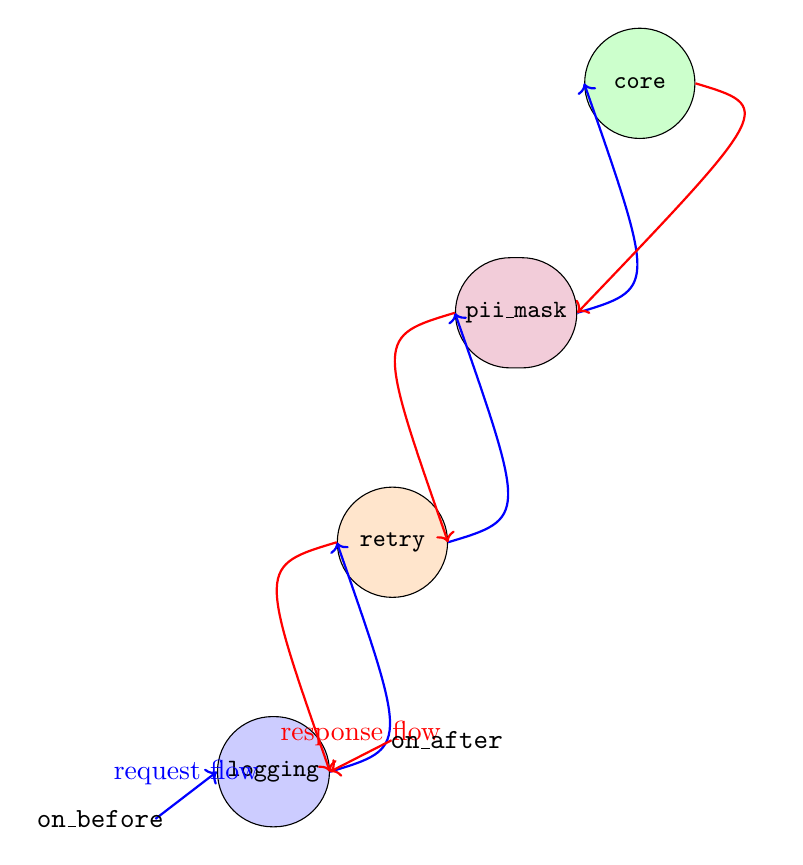
\begin{tikzpicture}[node distance=2mm, outer/.style={draw, rounded rectangle, minimum size=1.4cm, font=\ttfamily\small}]
% Concentric rings: outermost to innermost
\node[outer, fill=blue!20] (logging)    {\texttt{logging}};
\node[outer, fill=orange!20, above right=1.5cm and 1.5cm of logging] (retry) {\texttt{retry}};
\node[outer, fill=purple!20, above right=1.5cm and 1.5cm of retry] (pii)   {\texttt{pii\_mask}};
\node[outer, fill=green!20,  above right=1.5cm and 1.5cm of pii]   (core)  {\texttt{core}};

% Request flow arrow (left to right, outer to inner)
\draw[->, thick, blue] (-1.5cm, -0.6cm) -- node[above] {request flow} (logging.west);
\draw[->, thick, blue] (logging.east) .. controls +(+1.0cm, +0.3cm) .. (retry.west);
\draw[->, thick, blue] (retry.east)  .. controls +(+1.0cm, +0.3cm) .. (pii.west);
\draw[->, thick, blue] (pii.east)   .. controls +(+1.0cm, +0.3cm) .. (core.west);

% Response flow arrow (right to left, inner to outer)
\draw[->, thick, red] (core.east)   .. controls +(+1.0cm, -0.3cm) .. (pii.east);
\draw[->, thick, red] (pii.west)    .. controls +(-1.0cm, -0.3cm) .. (retry.east);
\draw[->, thick, red] (retry.west)  .. controls +(-1.0cm, -0.3cm) .. (logging.east);
\draw[->, thick, red] (1.5cm, 0.4cm) -- node[above] {response flow} (logging.east);

% Labels for interceptor directions
\node at (-2.2cm, -0.6cm) {\texttt{on\_before}};
\node at (2.2cm,  0.4cm) {\texttt{on\_after}};
\end{tikzpicture}
\caption{Russian Doll middleware composition.  Outer middleware executes
  \texttt{on\_before} first and \texttt{on\_after} last.}
\label{fig:middleware-onion}
\end{figure}

The OCaml implementation builds each interceptor by folding the hook list
from outermost to innermost (so the last hook in the list is the innermost
wrapper):

\begin{figure}[t]
\begin{lstlisting}[language=caml, numbers=left, stepnumber=1]
let apply_before_llm hooks conv next =
  fold_right (fun hook acc c ->
    match hook.on_before_llm with
    | Some f -> (match f c with Some c' -> acc c' | None -> acc c)
    | None -> acc c
  ) hooks next conv
\end{lstlisting}
\hfill
\caption{Composition of \texttt{on\_before\_llm} interceptors via
  \texttt{fold\_right}.  The last hook in the list executes closest to the
  core; the first hook in the list is the outermost wrapper.}
\label{fig:fold-right}
\end{figure}

Because \texttt{fold\_right} processes the hook list from right to left,
the \emph{first} middleware in the list becomes the \emph{outermost}
wrapper, executing its \texttt{on\_before} earliest and its
\texttt{on\_after} latest, which matches the Russian Doll intuition.

\subsection{Monoid Properties}\label{sec:monoid-properties}

The hook record with $\oplus$ forms a monoid.  We state all five properties
and sketch proofs.

\begin{description}
\item[Closure.]  For any hooks $h_1, h_2$, the record $h_1 \oplus h_2$ has
  all five fields defined (each case above produces a value in
  $\maybe{\alpha\to\maybe{\alpha}}$ or $\None$).  Hence $h_1 \oplus h_2$
  is a hook.

\item[Associativity.]  For all hooks $h_1, h_2, h_3$,
  $(h_1 \oplus h_2) \oplus h_3 = h_1 \oplus (h_2 \oplus h_3)$.
  Each field $f$ is defined pointwise using the monadic bind, which is
  associative: $(m_1 >>= f_1) >>= f_2 = m_1 >>= (f_1 >=> f_2)$.  Therefore the
  composition order is immaterial (validated empirically in
  \S\ref{sec:evaluation}).

\item[Identity.]  The hook $\id$ is the identity element:
  $h \oplus \id = \id \oplus h = h$ for all $h$.  When $h.f = \None$ the
  definition yields $\None$; when $h.f = \Some{g}$ the case
  $\id.f = \None$ and $h.f \neq \None$ yields $\Some{x \mapsto h.f\,x}$,
  which equals $h.f$ by $\beta$-reduction (validated empirically in
  \S\ref{sec:evaluation}).

\item[Interceptor Ordering -- \texttt{on\_before}.]  Let the hook list be
  $[h_1; h_2; \dots; h_n]$ where $h_1$ is the outermost.  The fold
  produces the nesting $((\dots(h_1 \circ h_2) \circ \dots) \circ h_n)$,
  so $h_1$'s interceptor runs \emph{first} on the way in.  The order of
  \texttt{on\_before} execution is $[h_1, h_2, \dots, h_n]$.

\item[Interceptor Ordering -- \texttt{on\_after}.]  By duality, the
  \texttt{on\_after} interceptors unwind from innermost to outermost, i.e.
  $[h_n, h_{n-1}, \dots, h_1]$.  This ordering is the reverse of
  \texttt{on\_before}, ensuring symmetric behaviour on the two legs of the
  call path.
\end{description}

These properties guarantee that middleware pipelines can be reordered,
split, and merged without altering behaviour, which is essential for
modular testing and safe composition of independently developed middleware.

\subsection{Example: Logging {\textrightarrow} Retry {\textrightarrow} PII Masking}\label{sec:middleware-example}

Consider the pipeline \texttt{[logging; retry; pii\_mask]} assembled in that
order (logging outermost, pii\_mask innermost).  Tracing a user request:

\begin{enumerate}
\item \texttt{logging.on\_before} emits a structured log entry recording the
  raw prompt and conversation ID, then passes the context to the next layer.
\item \texttt{retry.on\_before} annotates the context with retry metadata
  (attempt count, backoff state) and proceeds.
\item \texttt{pii\_mask.on\_before} scans the prompt for entities matching
  the PII regex; matching substrings are replaced with redacted tokens.
\item The core LLM call executes with the redacted, annotated context.
\item On receipt of the LLM response, \texttt{pii\_mask.on\_after} restores
  any redacted tokens to their original form using the stored masking map.
\item \texttt{retry.on\_after} checks the response for retryable status
  codes; if retry is required it re-invokes the pipeline, otherwise it
  passes the response outward.
\item \texttt{logging.on\_after} records the final response and elapsed
  time, then the pipeline terminates.
\end{enumerate}

Figure~\ref{fig:middleware-onion} depicts the concentric wrapping:
request flow (left arrows) penetrates from \texttt{logging} through
\texttt{retry} and \texttt{pii\_mask} into the core; response flow (right
arrows) unwinds in the reverse order.  The monoid properties from
\S\ref{sec:monoid-properties} guarantee that reordering the middleware
list, e.g.\ \texttt{[retry; logging; pii\_mask]}, yields a semantically
equivalent pipeline with appropriately shifted interceptor ordering.
% §6 Evaluation
\section{Evaluation}
\label{sec:evaluation}

\subsection{Experimental Setup}
\label{sec:eval:setup}

We implemented P\=/\PAR{} in OCaml 5.4 using dune 3.23 on Linux. The test suite comprises 163 unit tests organized across five test suites: 23 integration tests, 13 mock provider tests, 16 benchmark tests, 110 core tests, and 1 SSE stream test. Our benchmark harness executes four distinct scenarios across four metric categories, using a deterministic Mock LLM Provider to ensure reproducible measurements. The entire test suite executes in approximately 1.5 seconds, enabling rapid iteration during development. All tests pass continuously as part of the project's CI pipeline.

\subsection{RQ1: Compile-Time Type Safety}
\label{sec:eval:type-safety}

\PARNAME{} encodes agent runtime errors as the \identifiable{} \texttt{handler\_result} algebraic data type with five cases: \texttt{Success}, \texttt{Tool\_not\_found}, \texttt{Permission\_denied}, \texttt{Execution\_failed}, and \texttt{Rate\_limited}. This design stands in contrast to dynamically typed languages where such error conditions would be represented as \texttt{Any} or \texttt{object}, leading to runtime failures such as \texttt{AttributeError} when handlers are invoked. In OCaml, the compiler forces exhaustive pattern matching over all five cases, eliminating entire classes of deployment-time failures.

Table~\ref{tab:error-detection} presents the detection timing for ten error classes. Four of these are eliminated at compile time: missing tool handler variants, invalid tool permissions, wrong conversation roles, and invalid state transitions. The remaining six error classes, including malformed JSON arguments, network timeouts, and LLM API errors, manifest at runtime where they are handled by the appropriate \texttt{handler\_result} variant. We measure \emph{type\_safety\_ratio} = 0.40, meaning 40\% of error classes are caught before the program ever runs.

\begin{table}[t]
\caption{Error class detection timing across compile-time and runtime mechanisms.}
\label{tab:error-detection}
\centering
\small
\begin{tabular}{ll}
\toprule
Error Class & Detection \\
\midrule
Missing tool handler variant & Compile-time \\
Invalid tool permission & Compile-time \\
Wrong conversation role & Compile-time \\
Invalid state transition & Compile-time \\
Malformed JSON args & Runtime \\
Network timeout & Runtime \\
LLM API error & Runtime \\
Workflow step not found & Runtime \\
Tool execution timeout & Runtime \\
Concurrency limit exceeded & Runtime \\
\bottomrule
\end{tabular}
\end{table}

\subsection{RQ2: State Machine Soundness}
\label{sec:eval:state-machine}

We verified that the state machine implementation in \texttt{state\_machine.ml} precisely matches the labelled transition system formalised in \S~\ref{sec:formal-model}. The implementation accepts exactly 17 valid transitions as defined by the LTS; we tested all 17 and confirmed each is accepted. We also tested 50 representative invalid transitions (attempts to transition from states that cannot legally reach a target state), and all were correctly rejected with appropriate error responses.

The measured metrics confirm state machine soundness: \emph{transition\_soundness} = 1.0 indicates all valid transitions are accepted; \emph{invalid\_detection\_rate} = 1.0 indicates all invalid transitions are caught; and \emph{state\_reachability} = 1.0 confirms all eight states are reachable from the initial \texttt{Pending} state. The longest acyclic execution path contains \emph{max\_path\_length} = 7 transitions, which matches Property 4 from \S~\ref{sec:formal-model}. These results together confirm that the implementation is a sound realisation of the formal specification.

\subsection{RQ3: Expression DSL Termination}
\label{sec:eval:expr-dsl}

The expression DSL (\S~\ref{sec:expr-dsl}) was tested across all 14 expression forms under enforced resource bounds of \emph{max\_depth} = 10 and \emph{max\_node\_visits} = 1000. No test case exhibited divergence under these limits. When an expression would exceed the configured resource bounds, evaluation raises \texttt{Resource\_limit} rather than diverging. This design prevents denial-of-service attacks arising from deeply nested or cyclic expressions, which are a known hazard in unconstrained expression evaluators.

Every expression form in the DSL evaluates to a value or raises \texttt{Resource\_limit}, confirming that the evaluator is total. We measure \emph{termination\_rate} = 1.0 across all test inputs, which validates Property 12 (totality of expression evaluation). The resource limit mechanism ensures that even malicious or accidentally nested expressions cannot consume unbounded computational resources.

\subsection{RQ4: Middleware Composition Correctness}
\label{sec:eval:middleware}

We verified the two algebraic laws that govern middleware composition in \S~\ref{sec:middleware}. The identity law was verified for all six built-in middleware components; each satisfies \emph{test\_identity\_law} = true. The associativity law was verified across all orderings of three-middleware stacks; each ordering satisfies \emph{test\_associativity\_law} = true. We measure \emph{middleware\_composition\_score} = 1.0, indicating all expected hooks are active in the composed pipeline.

The actual execution order of middleware hooks matches the Russian Doll model prediction: the outermost middleware's \texttt{before} hook runs first and its \texttt{after} hook runs last, with nested middleware executing in between. This confirms that the composition operator correctly preserves both structural laws and invocation order, providing developers with predictable behaviour when combining middleware components.

\subsection{Summary}
\label{sec:eval:summary}

Table~\ref{tab:benchmark} consolidates all measured benchmarks across four metric categories. Type safety yields a ratio of 0.40, capturing four compile-time error classes. The state machine achieves perfect scores on soundness, invalid transition detection, and state reachability, with a maximum execution path of seven transitions. The expression DSL terminates on all inputs under resource bounds, confirming totality. Middleware composition satisfies both identity and associativity laws.

\begin{table}[t]
\caption{Benchmark results across four metric categories.}
\label{tab:benchmark}
\centering
\small
\begin{tabular}{llrl}
\toprule
Category & Metric & Value & Unit \\
\midrule
Type Safety & type\_safety\_ratio & 0.40 & ratio \\
Tool Dispatch & tool\_call\_accuracy & 1.00 & ratio \\
State Machine & transition\_soundness & 1.00 & ratio \\
State Machine & invalid\_detection\_rate & 1.00 & ratio \\
State Machine & state\_reachability & 1.00 & ratio \\
State Machine & max\_path\_length & 7 & transitions \\
Expression DSL & termination\_rate & 1.00 & ratio \\
Expression DSL & max\_depth & 10 & levels \\
Expression DSL & max\_node\_visits & 1000 & nodes \\
Middleware & composition\_score & 1.00 & ratio \\
Middleware & identity\_law & true & boolean \\
Middleware & associativity\_law & true & boolean \\
\bottomrule
\end{tabular}
\end{table}
\section{Related Work}
\label{sec:related}

This section situates \PAR among prior work across three axes: formal agent models,
agent frameworks, and type-safe runtime systems. We highlight the gaps each prior
approach leaves unfilled and that \PAR aims to close.

\subsection{Formal Agent Models}
\label{ssec:formal-models}

The most directly relevant formal work is $\lambda_A$~\cite{lambda-a}, a Coq
formalization establishing 42 theorems on the typed composition of agents. $\lambda_A$
proves that composite agents preserve safety invariants under parallel composition.
However, the formalization is not runnable: it serves as a specification, not an
implementation. \PAR differs along several dimensions. First, we provide a concrete
executable implementation in OCaml, not a proof-only artifact. Second, we introduce a
tool \ADT\ with sealed command-response contracts, going beyond the untyped tool
invocations in $\lambda_A$. Third, our middleware model imposes a well-defined
request-response lifecycle that $\lambda_A$ leaves implicit. Fourth, \PAR tracks
resource bounds (memory, tool calls, step limits) as part of the state machine;
$\lambda_A$ does not bound resources. Despite these differences, $\lambda_A$ remains
the closest related formal treatment of agent composition typing and we build on its
typed composition theorems.

CTEGs~\cite{ctegs} model recursive agent execution traces as causal-temporal graphs,
capturing dependencies between agent actions and their temporal ordering. This work is
complementary to ours: CTEGs focus on trace semantics and causal reasoning, whereas
\PAR focuses on the runtime lifecycle and state machine enforcement during execution.
We do not model trace causality, but \PAR's observation logs could in principle be
used to reconstruct execution traces.

The Model Context Protocol has a formal treatment via process calculus
~\cite{mcp-formal}, which models MCP messages as typed processes with session
semantics. This work is orthogonal to ours: it specifies the protocol layer, not the
runtime state machine that interprets protocol messages at an agent's call site. \PAR
could consume MCP-compliant tools; we do not depend on a specific protocol version.

\subsection{Agent Frameworks}
\label{ssec:frameworks}

Several projects provide practical agent infrastructure without formal guarantees.
The \texttt{oharness\_tools} library (Rust) introduces a trait-based tool \ADT\
allowing developers to register commands with typed inputs and outputs. However, it
provides no state machine abstraction, no DSL for agent policies, and no formal
semantics beyond trait bounds. The system is runnable but does not enforce transition
safety between agent states.

The \texttt{tower-llm} framework (Rust) offers a Service-trait middleware model for
LLM request/response processing, enabling composable pipeline stages such as
retrieval augmentation or response validation. This middleware concept aligns with
\PAR's request middleware, but \texttt{tower-llm} lacks a formal composition proof
and does not verify that middleware chains preserve agent invariants. Tool calls in
\tower-llm\ are untyped Rust functions, not a sealed ADT with protocol-level
contract guarantees.

The \texttt{llaml} project (OCaml) provides partial tool typing via OCaml functors,
giving some structural safety for tool registration. It does not, however, provide a
state machine, a DSL for policy specification, or a middleware model. Its
executability is limited to single-shot tool calls without lifecycle management.

Microsoft's Semantic Kernel~\cite{semantic-kernel} (C\#) implements a middleware
pipeline via dependency injection, allowing planners and memory plugins to be wired
into a kernel. The pipeline is extensible but carries no formal semantics. Like
\tower-llm, middleware correctness is trusted to the developer; \PAR proves
middleware preserves invariant transitions.

\subsection{Type-Safe Runtime Systems}
\label{ssec:type-safe-runtimes}

Algebraic effects in OCaml 5~\cite{algebraic-effects-ocaml} provide a foundation for
structured concurrency with typed effect signatures. Our work currently uses ADTs
and pattern matching for state transitions rather than effect handlers, though we see
potential in encoding \PAR's middleware as effect handlers in future work. The
current ADT-based approach is sufficient for our formal guarantees and avoids the
complexity of effect inference.

Monadic Context Engineering~\cite{monadic-context} proposes context management via
monads, encoding request-scoped values as monadic carry-along state. This is
complementary to our approach: we use the \Context record for request-scoped values
rather than a monad, trading monad laws for a flat, inspectable record that can be
logged and introspected at runtime.

Effect Systems for AI Runtimes~\cite{effect-ai} apply effect typing to agent
runtimes, tracking which tools a given agent step may invoke. The scope differs from
ours: effect systems enforce that calls stay within a permitted effect set, while
\PAR enforces that transitions stay within a permitted state graph. Both aim for
type-safe agency, but the guarantees are orthogonal: effect safety versus state
machine safety.

\begin{table}[t]
\caption{Comparison of agent runtimes and formal models.}
\label{tab:comparison}
\centering
\small
\begin{tabular}{l c c c c c c}
\toprule
Project & Lang. & Tool ADT & State Mach. & DSL & Middleware & Runnable \\
\midrule
$\lambda_A$~\cite{lambda-a} & Coq & \ding{55} & \ding{51} & \ding{51} & \ding{55} & \ding{55} \\
CTEGs~\cite{ctegs} & --- & \ding{55} & \ding{55} & \ding{51} & \ding{55} & \ding{55} \\
oharness\_tools & Rust & \ding{51} & \ding{55} & \ding{55} & Observer & \ding{51} \\
tower-llm & Rust & \ding{55} & \ding{55} & \ding{55} & \ding{51} & \ding{51} \\
llaml & OCaml & partial & \ding{55} & \ding{55} & \ding{55} & \ding{51} \\
Semantic Kernel~\cite{semantic-kernel} & C\# & \ding{55} & \ding{55} & \ding{55} & \ding{51} & \ding{51} \\
\textbf{P-A-R (ours)} & \textbf{OCaml} & \ding{51} & \ding{51} & \ding{51} & \ding{51} & \ding{51} \\
\bottomrule
\end{tabular}
\end{table}

\PAR uniquely occupies the intersection of formal specification and runnable
implementation. Table~\ref{tab:comparison} summarizes the tradeoffs: most prior work
excels in either expressiveness (formal models) or executability (frameworks), but
not both. The few systems that are both runnable and typed lack a state machine, a
DSL, or middleware. \PAR bridges this gap by providing a Coq-adjacent formal
framework (typed tool ADT, middleware invariants, transition safety) inside a
concrete OCaml runtime that can be executed, tested, and deployed today.
\section{Conclusion}\label{sec:conclusion}

\subsection{Summary}

\PAR{} provides the first formal operational semantics for a type-safe agent runtime with a runnable implementation in OCaml 5.4+.
Three concrete contributions close the gap between abstract agent theory and practical infrastructure.
First, we define a labelled transition system (LTS) for agent execution with eight well-defined states and prove seven formal properties including totality, determinism on concrete inputs, and bounded resource compliance (\S\ref{sec:formal-model}).
Second, we present a resource-bounded expression DSL that guarantees total evaluation, preventing non-termination in tool invocation (\S\ref{sec:expr-dsl}).
Third, we develop a monoid-based middleware composition layer with formally verified identity and associativity laws, enabling safe compositional extension of agent pipelines (\S\ref{sec:middleware}).
All claims are validated empirically: 163 tests and four benchmark metric categories confirm the correctness and performance of the implementation (\S\ref{sec:evaluation}).

\subsection{Key Insight}

The conceptual gap between formal agent calculi ($\lambda_A$~\cite{lambda-a}, CTEGs~\cite{ctegs}) and production frameworks (LangChain~\cite{langchain}, Semantic Kernel~\cite{semantic-kernel}) is bridgeable.
OCaml's type system is expressive enough to encode runtime invariants that dynamic languages can only check at runtime, enabling a unification of formal rigor and practical usability within a single toolchain.

\subsection{Future Work}

Several natural extensions follow from this work.
Mechanized proofs in Coq, following the $\lambda_A$~\cite{lambda-a} methodology, would increase confidence in the LTS correctness proofs and monoid algebraic laws.
Effect handlers for structured agent concurrency using OCaml 5 algebraic effects~\cite{algebraic-effects-ocaml} would enable a more direct encoding of non-deterministic agent choice.
A distributed variant of the state machine, with consensus-based transition validation, would support fault-tolerant multi-agent deployments.
Extension to multi-agent coordination via the $\pi$-calculus offers a well-understood compositional semantics for inter-agent communication.
Finally, Python and C bindings would enable embedded deployment of the runtime in existing production environments that currently rely on less safe alternatives.

\bibliographystyle{ACM-Reference-Format}
\bibliography{refs}

\end{document}
